\documentclass[12pt]{report}
\usepackage[a4paper,margin=1in]{geometry}
\usepackage{setspace} % for single/doublespacing commands
\usepackage{graphicx} % including graphics
\usepackage{sectsty} % sexy section headings
\usepackage{pdfpages} % including multipage pdfs
\usepackage[export]{adjustbox} % for graphic frames and center
\usepackage{amssymb} % special math symbols
\usepackage{cancel} % arrow and cross math cancel symbol
\usepackage[numbered]{matlab-prettifier} % including matlab w/ syntax highlighting
\usepackage[T1]{fontenc} % prettier matlab font
\usepackage{circuitikz} % drawing fancy shit
\usepackage{xfrac} % more legible inline fractions (\sfrac)
\usepackage{lmodern} % font package for above
\usepackage{multicol} % multiple columns
\usepackage[justification=centering]{caption} % figure captions (force centering)
\usepackage{amsmath} % more math symbols and shit
\usepackage{enumitem} % add arguments for enumerate to change style
\usepackage[list=true]{subcaption} % subfigures with list of figure support

\newcommand{\eqname}[1]{\tag*{#1}}% Tag equation with name

\lstMakeShortInline[style=Matlab-editor]| % matlab inline escape character
\usetikzlibrary{arrows}
\usetikzlibrary{decorations.pathmorphing} % for snakes! Meow
\graphicspath{{images/}}
\usetikzlibrary{calc,patterns,angles,quotes}

\allsectionsfont{\centering}
\renewcommand\thesection{\arabic{section}}
\renewcommand{\thefootnote}{\arabic{footnote}}
\setcounter{tocdepth}{3}

\begin{document}

\input{titlepage}
\pagenumbering{roman}
{\tableofcontents\let\clearpage\relax\listoffigures}
\clearpage
\pagenumbering{arabic}
\newpage
\begin{flushleft}

% ---------------------------------------------------------------------------- %
\section{Conceptualize the Problem}
% ---------------------------------------------------------------------------- %


\begin{figure}[h]
  \begin{minipage}[c]{.45\textwidth}
  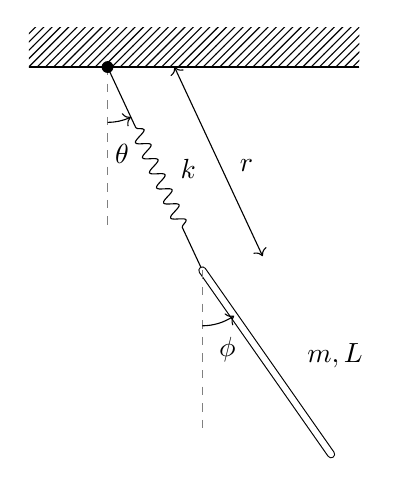
\begin{tikzpicture}

  \pgfmathsetmacro{\Gvec}{1.5}
  \pgfmathsetmacro{\myAngle}{25}

  \coordinate (centro) at (0,0);
  \draw[dashed,gray,-] (centro) -- ++ (0,-2) node (vert1) [black,below]{$ $};

  \draw (centro) -- ++(270+\myAngle:.85) coordinate (spring1);
  \draw[decorate, decoration={snake, segment length=6, amplitude=2.4}] (spring1) -- ++(270+\myAngle:1.5) coordinate (spring);
  \draw (spring) -- ++(270+\myAngle:.5) coordinate (spring2);
  \pic [draw,angle radius=20,->, "$\theta~$", angle eccentricity=1.6] {angle = vert1--centro--spring};

  \draw[<->] (.85,0) -- ++(270+\myAngle:2.65) coordinate (r);
  \draw ($(.85,0) + (270+\myAngle:2.75/2)$) node[label=0:$r$] {};
  \draw ($(.25,0) + (270+\myAngle:2.75/1.5)$) node[label=$k$] {};


  \fill[pattern = north east lines] ($(-1,0)$) rectangle ($(3.2,0.5) $);
  \draw[thick] ($ (centro) + (-1,0) $) -- ($ (centro) + (3.2,0) $);

  \draw[double distance = .75mm,line cap=round] (spring2) -- ++(270+\myAngle+10:2.85) coordinate (bar);

  \draw ($ (bar) + (.05,1.25)$) node[label] {$m,L$};

  \draw[dashed,gray,-] (spring2) -- ++ (0,-2) node (vert2) [black,below] {};
  \pic [draw,angle radius=20,->, "$\phi$", angle eccentricity=1.5] {angle = vert2--spring2--bar};




  \fill[black] (centro) circle (0.075);
\end{tikzpicture}

\end{minipage}%
\begin{minipage}[c]{.55\textwidth}
  The pendulum system consists of a rigid bar pinned to the free end of a linear spring,
  which rotates about its opposite end at a fixed point.
\end{minipage}
\end{figure}

\subsection{Constants and Assumptions}
\begin{tabular}{ll@{\hskip .75in}l}
 \multicolumn{1}{c}{Constants:} && \multicolumn{1}{c}{Assumptions:} \\
 Bar Mass: &$m$ = 1 kg & No Losses\\
 Bar Length: &$L$ = 1 m & Released from Rest\\
 Gravity: &$g$ = 9.81$\sfrac{m}{s^2}$ &Slender Bar \\
 Linear Spring: &&Planar\\
 \quad Spring Coefficient:& $k = 25~\sfrac{N}{m}$ &Rigid-Body Dynamics \\
 \quad Unstretched Length:& $L$ = 0.5 m \\
\end{tabular}
\vspace{5ex}

We are asked to determine the following: \\
\begin{enumerate}
  \item The Equations of Motion for the system via the Lagrangian method.
  \item Integrate the Equations of Motion using various initial conditions and plot
  the behavior of the system for 10 seconds. \\
  \vspace{2ex}
  $
    \begin{array}{cll}
    \text{(a)} & \theta_o = 0~rad, & \phi_o = 0~rad \\
    \text{(b)} & \theta_o = \sfrac{\pi}{18}~rad, & \phi_o = \sfrac{\pi}{9}~rad \\
    \text{(c)} & \theta_o = \sfrac{\pi}{6}~rad, & \phi_o = \sfrac{\pi}{3}~rad \\
  \end{array}
  $
  \item Plot the total energy versus time for all 3 cases.
  \item Repeat 2. and 3. using a 'RelTol' of 1e-6 and 'AbsTol' 1e-9 for the
  |ode45| integration tolerances.
\end{enumerate}

% ---------------------------------------------------------------------------- %
\section{Free Body Diagram}
% ---------------------------------------------------------------------------- %

% ---------------------------------------------------------------------------- %
\section{Coordinate Frame} \label{section:coord}
% ---------------------------------------------------------------------------- %

% ---------------------------------------------------------------------------- %
\section{Sum of Forces}
% ---------------------------------------------------------------------------- %
% ---------------------------------------------------------------------------- %
\section{Constraints}
% ---------------------------------------------------------------------------- %
% ---------------------------------------------------------------------------- %
\section{Solve for the Equations of Motion}
% ---------------------------------------------------------------------------- %

\newpage
% ---------------------------------------------------------------------------- %
\section{Solve the Equations of Motion}
% ---------------------------------------------------------------------------- %
% ---------------------------------------------------------------------------- %
\section{Does it Make Sense?}
% ---------------------------------------------------------------------------- %
\subsection{Units}
Checking with the MATLAB symbolic units tool (from Section \ref{appendix:numerical}): \\
~\\
% \begin{lstlisting}[frame=lines,style=Matlab-editor]
% Checking EOM Units
u = symunit;
m2 = m2*u.kg;
k = k*u.N/u.m;
L0 = L0*u.m;
l2 = l2*u.m;
g = g*u.m/u.s^2;
thetat = 'thetat';
thetadot = 'thetadot'/u.s;
thetaddot = 'thetaddot'/u.s^2;
phit = 'phit';
phidot = 'phidot'/u.s;
phiddot = 'phiddot'/u.s^2;
l1t = 'l1t'*u.m;
l1dot = 'l1dot'*u.m/u.s;
l1ddot = 'l1ddot'*u.m/u.s^2;

eqn = subs(eqn)
unitCheck = checkUnits(eqn)
\end{lstlisting}
\color{gray} \begin{verbatim}
unitCheck =
  struct with fields:
    Consistent: [1 1 1]
    Compatible: [1 1 1]
\end{verbatim} \color{black}

\subsection{Magnitude}

\section{Appendix} \label{appendix}
\subsection{Attributions}
\onehalfspacing
\begin{tabular}{ll}
Jeffrey Chen & \\
Thorne Wolfenbarger &\\
Trey Dufrene & \\
Joint Effort &
\end{tabular}
\singlespacing

\newpage
\subsection{Analytical Solution}

\newpage
\subsection{Numerical Solution} \label{appendix:numerical}
% \begin{lstlisting}[frame=lines,style=Matlab-editor,basicstyle = \mlttfamily]

\end{lstlisting}


\end{flushleft}
\end{document}
